\chapter{11. Decorator Pattern}
\section{Giới thiệu}
\subsection{Đặt vấn đề}
Một trong những khía cạnh quan trọng nhất trong quá trình phát triển một ứng dụng mà các lập trình viên phải đối đầu là sự thay đổi. Khi muốn thêm hoặc loại bỏ một tính năng của một đối tượng, điều đầu tiên chúng ta nghĩ đến là thừa kế (extends). Tuy nhiên, thừa kế không khả thi vì nó là static, chúng ta không thể thêm các lớp con mới vào một chương trình khi nó đã được biên dịch và thực thi.\\
Để giải quyết vấn đề này, chúng ta có thể sử dụng Decorator Pattern. Mẫu thiết kế này sẽ linh động thay đổi tính chất (functionality) đã có trong một đối tượng khi chương trình đang chạy (runtime) mà không ảnh hưởng đến các tình chất đã tồn tại của các đối tượng khác.
\subsection{Mục đích sử dụng}
\begin{itemize}
    \item Tăng cường khả năng mở rộng của đối tượng, bởi vì những thay đổi được thực hiện bằng cách implement trên các lớp mới.
    \item Client sẽ không nhận thấy sự khác biệt khi bạn đưa cho nó một wrapper thay vì đối tượng gốc.
    \item Một đối tượng có thể được bao bọc bởi nhiều wrapper cùng một lúc.
    \item Cho phép thêm hoặc xóa tính năng của một đối tượng lúc thực thi (run-time).
\end{itemize}

\section{Định nghĩa và mô hình cấu trúc}
\subsection{Định nghĩa}
Decorator pattern là một trong những Pattern thuộc nhóm cấu  trúc (Structural). Nó cho phép người dùng thêm chức năng mới vào đối tượng hiện tại mà không muốn ảnh hưởng đến các đối tượng khác. Kiểu thiết kế này có cấu trúc hoạt động như một lớp bao bọc (wrap) cho lớp hiện có. Mỗi khi cần thêm tính năng mới, đối tượng hiện có được wrap trong một đối tượng mới (decorator class).\\
Decorator pattern sử dụng composition thay vì inheritance (thừa kế) để mở rộng đối tượng. Decorator pattern còn được gọi là Wrapper hay Smart Proxy.
\subsection{Mô hình cấu trúc}
\begin{figure}[!htb]
    \centering
    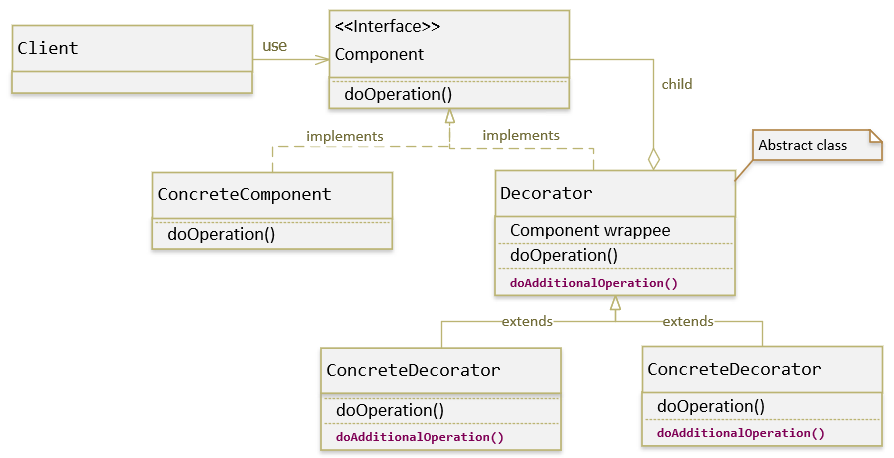
\includegraphics[width=\textwidth]{fig/Decorator/structure_decorator.png}
    \caption{Mô hình cấu trúc}
    \label{fig:structure_decorator}
\end{figure}
\newpage
\begin{itemize}
    \item Component: Là một interface quy định các phương thức chung cần phải có cho tất cả các thành phần tham gia vào mẫu này.
    \item ConcreteComponent: Là lớp thực hiện(implements) các phương thức của Component.
    \item Decorator: Là một abstract class dùng để duy trì một tham chiếu của đối tượng Component và đồng thời cài đặt các phương thức của Component  interface.
    \item ConcreteDecorator: Là lớp thực hiện các phương thức của Decorator, nó cài đặt thêm các tính năng mới cho Component.
    \item Client: Đối tượng sử dụng Component.
\end{itemize}

\section{Cách cài đặt}
Ví dụ cài đặt cho một hệ thống quản lý dự án, nơi nhân viên đang làm việc với các vai trò khác nhau, chẳng hạn như thành viên nhóm (team member), trưởng nhóm (team lead) và người quản lý (manager). Một thành viên trong nhóm chịu trách nhiệm thực hiện các nhiệm vụ được giao và phối hợp với các thành viên khác để hoàn thành nhiệm vụ nhóm. Mặt khác, một trưởng nhóm phải quản lý và cộng tác với các thành viên trong nhóm của mình và lập kế hoạch nhiệm vụ của họ. Tương tự như vậy, một người quản lý có thêm một số trách nhiệm đối với một trưởng nhóm như quản lý yêu cầu dự án, tiến độ, phân công công việc.

Sau đây là các thành phần tham gia vào hệ thống và hành vi của chúng:
\begin{itemize}
    \item Employee: Thực hiện công việc (doTask), tham gia vào dự án (join), rời khỏi dự án (terminate).
    \item Team member: Báo cáo task được giao (report task), cộng tác với các thành viên khác (coordinate with others).
    \item Team leader: Lên kế hoạch (planning), hỗ trợ các thành viên phát triển (motivate), theo dõi chất lượng công việc và thời gian (monitor).
    \item Manager: Tạo các yêu cầu dự án (create requirement), giao nhiệm vụ cho thành viên (assign task), quản lý tiến độ dự án (progress management).
\end{itemize}
Tiếp theo là mô hình cấu trúc áp dụng Decorator Pattern
\begin{figure}[!htb]
 \centering
 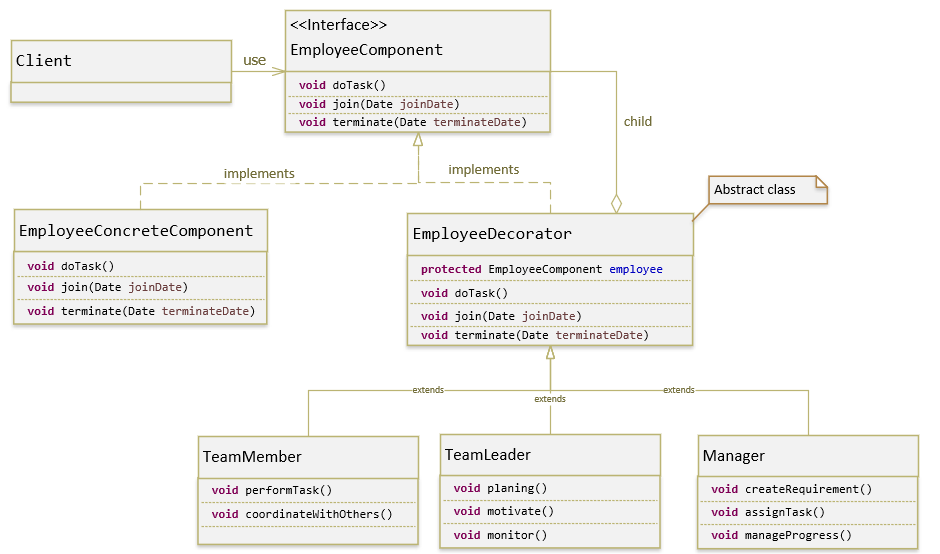
\includegraphics[width=\textwidth]{fig/Decorator/decorator_example.png}
 \caption{Mô hình cấu trúc quản lí dự án}
 \label{fig:decorator_example}
\end{figure}
 

Dưới đây là code của cài đặt.\\
Link code cài đặt: \url{https://github.com/nanhus/OOP-DesginPatten/tree/master/source/decorator}
\newpage
\begin{figure}[!htb]
    \centering
    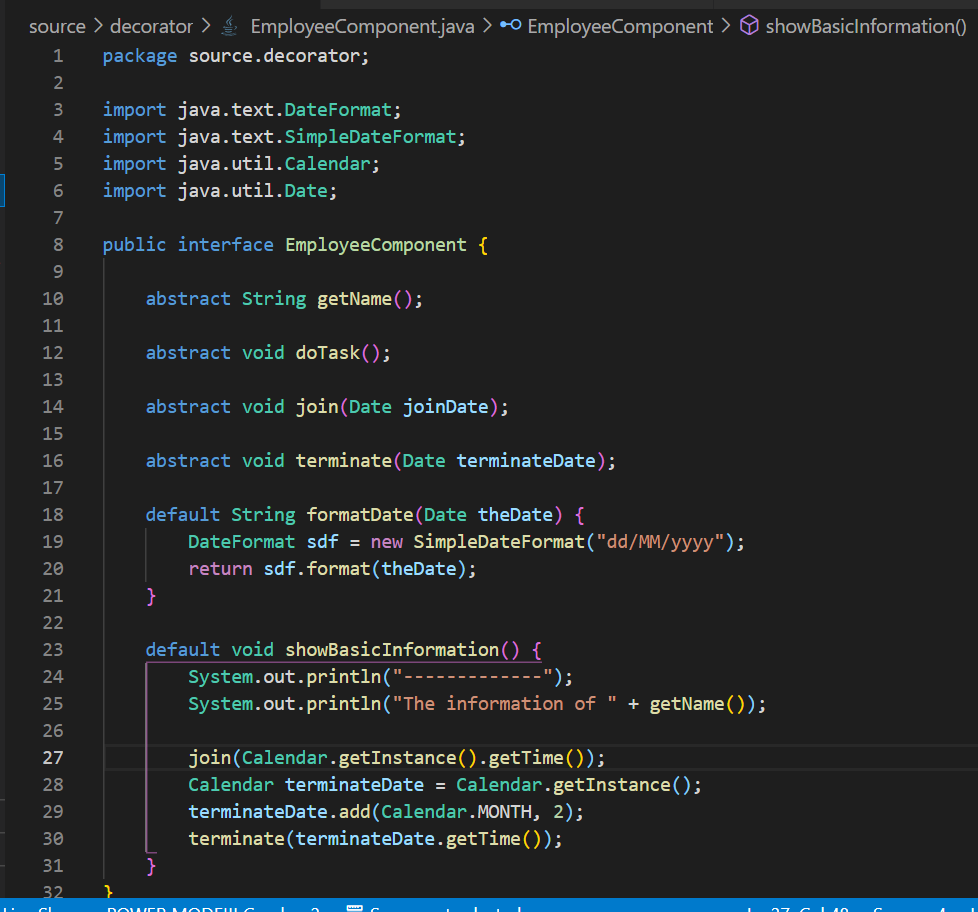
\includegraphics[width=\textwidth]{fig/Decorator/employee_component_interface.png}
    \caption{Employee Component Interface}
    \label{fig:employee_component_interface}
\end{figure}
\newpage
\begin{figure}[!htb]
    \centering
    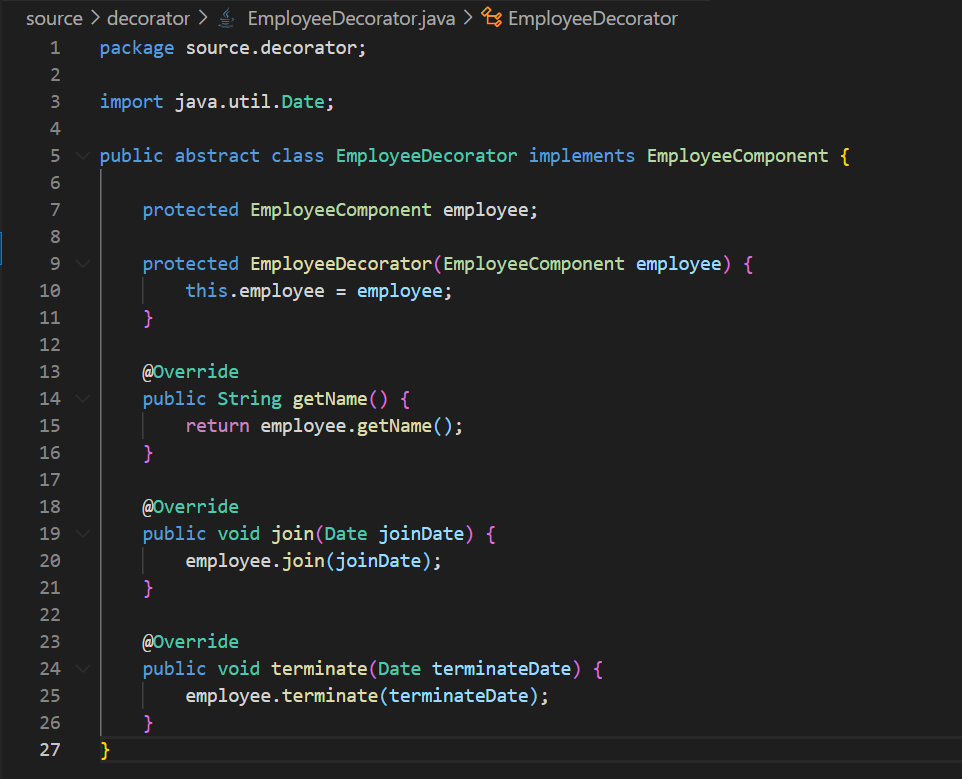
\includegraphics[width=\textwidth]{fig/Decorator/employee_decorator_class.png}
    \caption{Employee Decorator Class}
    \label{fig:employee_decorator_class}
\end{figure}
\newpage
\begin{figure}[!htb]
    \centering
    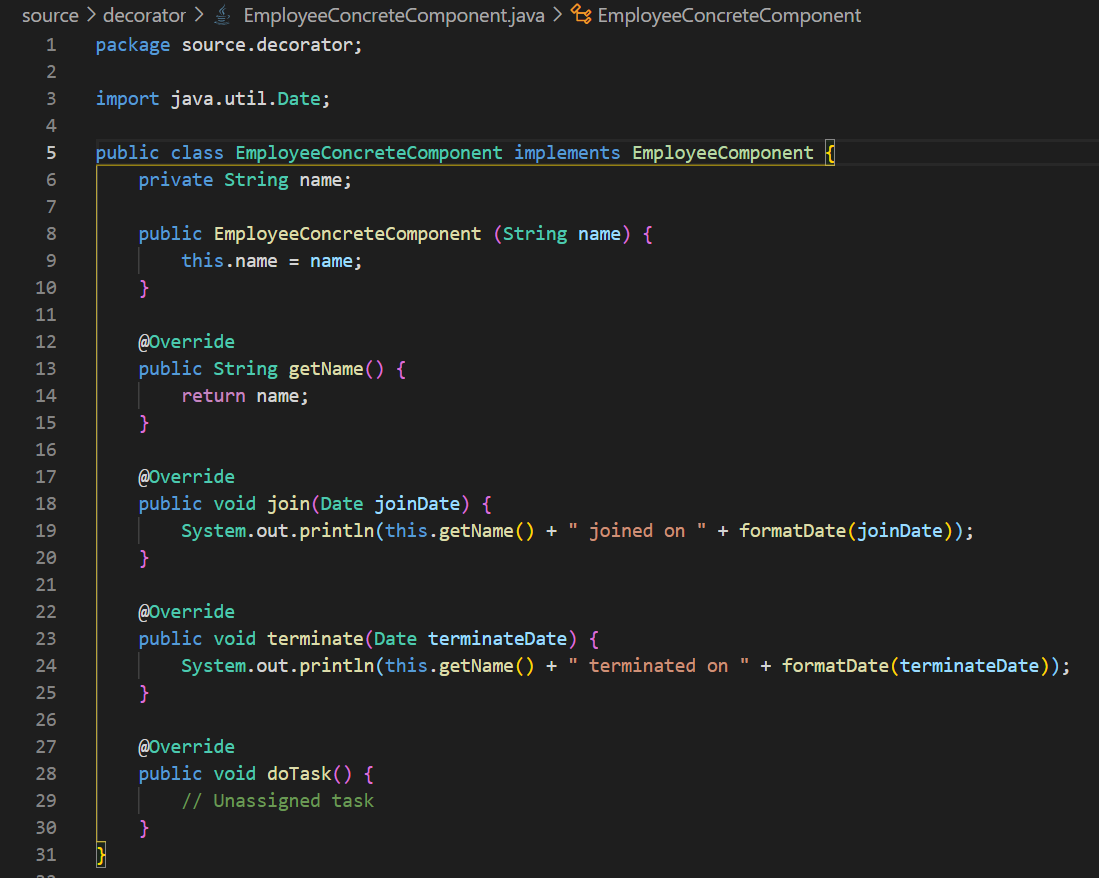
\includegraphics[width=\textwidth]{fig/Decorator/employee_concrete_component_class.png}
    \caption{Employee Concrete Component Class}
    \label{fig:employee_concrete_component_class}
\end{figure}

\begin{figure}[!htb]
    \centering
    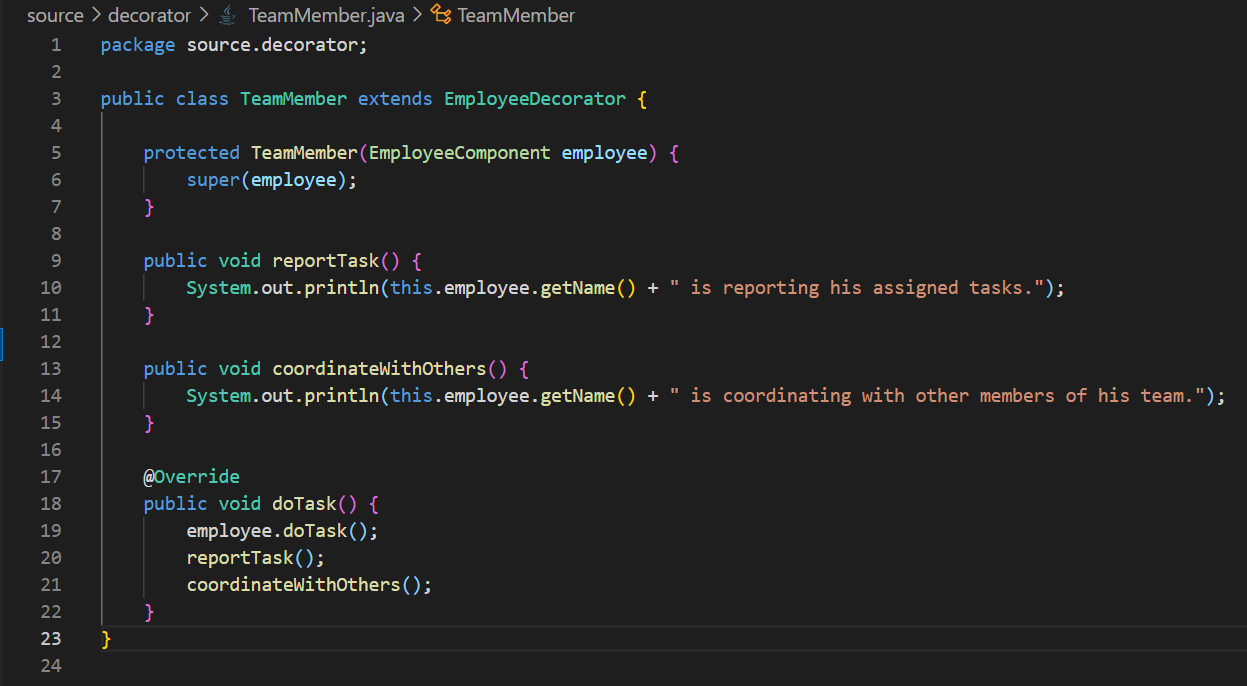
\includegraphics[width=\textwidth]{fig/Decorator/team_member_class.png}
    \caption{Team Member Class}
    \label{fig:team_member_class}
\end{figure}
\begin{figure}[!htb]
    \centering
    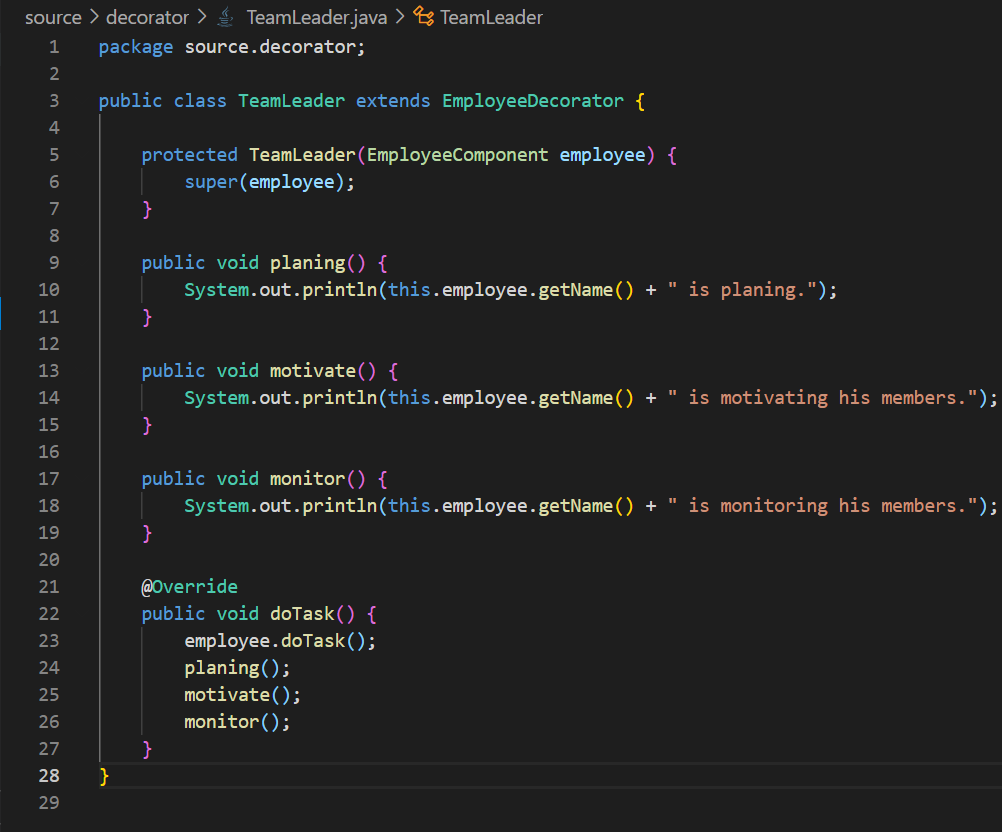
\includegraphics[width=\textwidth]{fig/Decorator/team_leader_class.png}
    \caption{Team Leader Class}
    \label{fig:team_leader_class}
\end{figure}
\newpage
\begin{figure}[!htb]
    \centering
    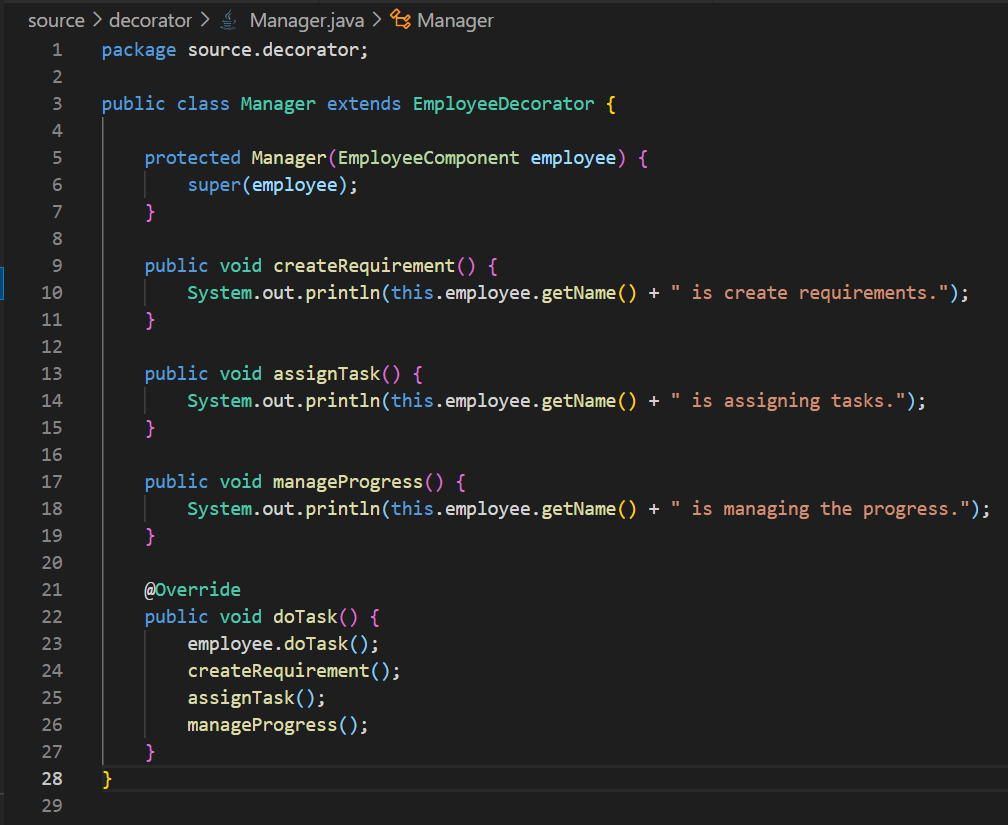
\includegraphics[width=\textwidth]{fig/Decorator/manager_class.png}
    \caption{Manager Class}
    \label{fig:manager_class}
\end{figure}
\newpage
\begin{figure}[!htb]
    \centering
    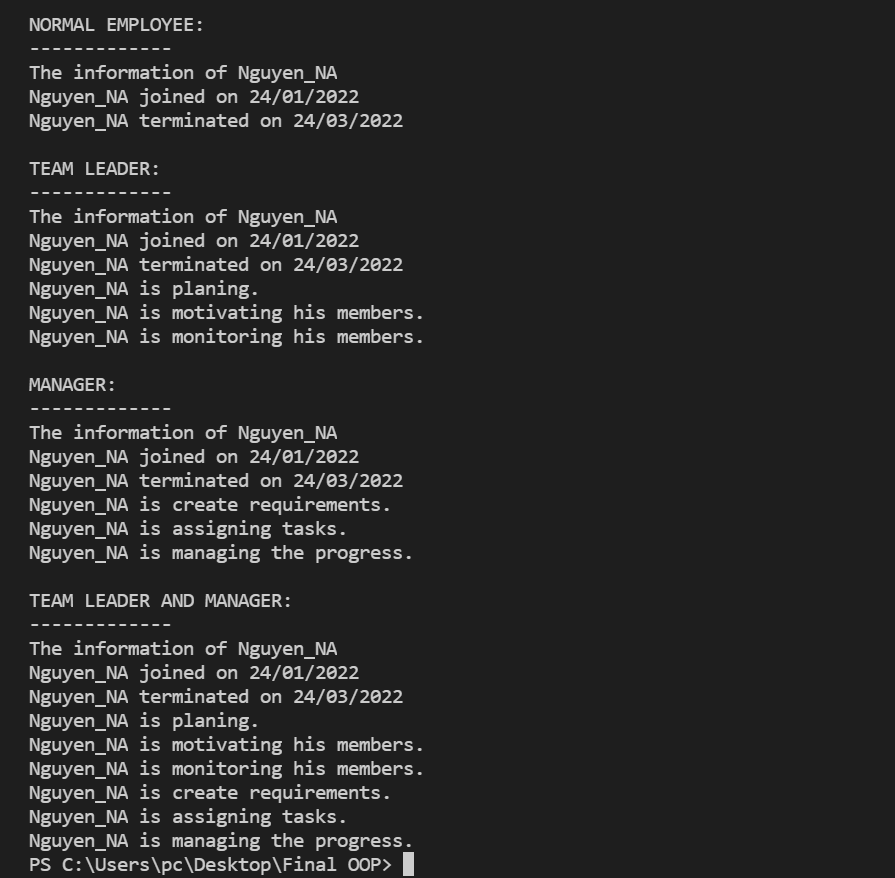
\includegraphics[width=\textwidth]{fig/Decorator/decorator_output.png}
    \caption{Output}
    \label{fig:decorator_output}
\end{figure}


\section{Ví dụ thực tế}
\begin{itemize}
    \item Tổ chức các API
    \item Quản lí nhân viên, hàng hóa
    \item Sử dụng trong lập trình đa luồng
    \item Decorator có trách nhiệm bổ sung vào một đối tượng một cách động. Ví dụ những đồ trang trí được thêm vào cây thông như đèn, vòng hoa, kẹo, đồ trang trí bằng thủy tinh, v.v.,
    \item Nhiều bộ công cụ giao diện người dùng hướng đối tượng sử dụng decorator để thêm phần tô điểm đồ họa cho các vật dụng. Ví dụ bao gồm Interviews [LVC89, LCI+92], ET++ [WGM88], và lớp thư viện ObjectWorks/Smalltalk [Par90].
    \item Stream là yếu tố cơ bản trong hầu hết chức năng I/O. Steam cung cấp một interface để chuyển đổi đối tượng thành một chuỗi các byte hoặc kí tự. Điều này cho phép ta chuyển dịch một đối tượng thành file hoặc string trong bộ nhớ để truy xuất sau này. Một cách đơn giản để thực hiện việc này là định nghĩa lớp trừu tượng Stream với những lớp con MemoryStream và FileStream. Giả sử ta muốn:
    \begin{itemize}
        \item Nén một lường dữ liệu sử dụng nhiều thuật toán nén khác nhau (run-length encoding, Lempel-Ziv,...)
        \item Giảm luồng dữ liệu thành các kí tự ASCII 7-bit để nó có thể được truyền đi qua kênh giao tiếp ASCII
    \end{itemize}
    Decorator Pattern cho ta một cách tao nhã để xử lý việc này vào những luồng. Lược đồ dưới đây là giải pháp của vấn đề kể trên:\\
    \begin{figure}[!htb]
        \centering
        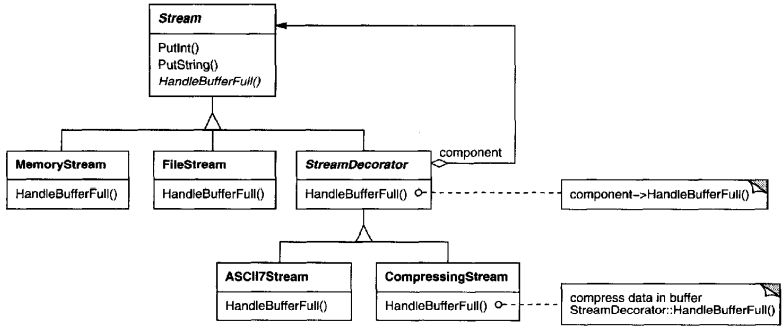
\includegraphics[width=\textwidth]{fig/Decorator/hmm.png}
    \end{figure}
    
    Lớp trừu tượng Stream duy trì một buffer bên trong và cung cấp các thao tác cho việc lưu trữ dữ liệu vào luồng (Putlnt,PutString). Mỗi khi buffer đầy, Stream sẽ gọi thao tác trừu tượng HandleBufferFull, thao tác này thực hiện việc truyền dữ liệu. Phiên bản FileStream của thao tác này sẽ ghi đè thao tác đó để chuyển buffer vào một tệp\\[0.1in]
    Lớp có vai trò chính ở đây là StreamDecorator, lớp này duy trì một tham chiếu tới một luồng thành phần và chuyển tiếp yêu cầu tới nó. Các lớp con của StreamDecorator ghi đè HandleBufferFull và thực hiện các hành động bổ sung trước khi gọi thao tác HandleBufferFull của StreamDecorator\\
    Ví dụ, lớp con CompressingStream nén dữ liệu và ASCII7Stream chuyển đổi dữ liệu thành 7-bit ASCII. Giờ để tạo một FileStream mà nén dữ liệu của nó và chuyển đổi dữ liệu nhị phân nén được thành 7-bitASCII, ta decorate FileStream với CompressingStream và ASCII7Stream:
    \begin{figure}[!htb]
        \centering
        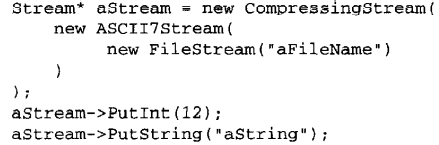
\includegraphics[width=\textwidth]{fig/Decorator/hmm2.png}
    \end{figure}
\end{itemize}
